\documentclass{article}
\usepackage[none]{hyphenat}  % Stop silly word wrapping
\usepackage{graphicx} % Required for inserting images
\usepackage{tikz}
\usepackage{pgfplots}
\pgfplotsset{compat=1.18}
\usepackage{placeins}


\title{Query Processing System Report}
\author{Jairik "JJ" McCauley}
\date{\today}

\begin{document}

\maketitle

\section{Samples}
For benchmarking query execution runtimes and computing performance measurements, timing samples were collected for each implementation (Serial, OpenMP, and OpenMPI) using dataset sizes of 50{,}000 and 1{,}000{,}000 records. For performance metrics, serial implemented were sampled 3 times to improve overall consistency/edge cases, while parallel implementations were tested using 1, 2, 4, and 6 cores. Additionally, all runtimes are measured in \textit{seconds}.

\subsection*{Serial Runtime Samples}

\begin{center}
\begin{tabular}{c c}
\hline
\textbf{50k} & \textbf{1M} \\
\hline
0.0219 & 2.7390 \\
0.0782 & 2.8672 \\
0.0532 & 2.7462 \\
\hline
\end{tabular}
\end{center}

\textit{Average for 1{,}000{,}000 Tuples}: $2.7841s$

\subsection*{OpenMP Runtime Samples}

\begin{center}
\begin{tabular}{c c c}
\hline
\textbf{Cores} & \textbf{50k} & \textbf{1M} \\
\hline
1 & 0.0229 & 0.7121 \\
2 & 0.0218 & 0.6795 \\
4 & 0.0222 & 0.5826 \\
6 & 0.0243 & 0.4979 \\
\hline
\end{tabular}
\end{center}


\subsection*{OpenMPI Runtime Samples}

\begin{center}
\begin{tabular}{c c c}
\hline
\textbf{Cores} & \textbf{50k} & \textbf{1M} \\
\hline
1 & 0.0192 & 0.5706 \\
2 & 0.0113 & 0.3645 \\
4 & 0.0133 & 0.2894 \\
6 & 0.0143 & 0.2292 \\
\hline
\end{tabular}
\end{center}


\subsection*{Potential Limitations}

Due to the complexity of the data (many features and indexes), the dataset sizes were limited when testing. In a real-world scenario (which I unfortunately could not implement), these datasets would be stored on the disk and not in memory, greatly reducing the cold-start runtimes (as data would be saved to disk as B+ trees) and total capabilities (current implementation must load everything into memory). While a 20{,}000{,}000 sample dataset was created for benchmarking, it unfortunately took too long when testing to be included within these samples.

This invokes limitations within the results, as smaller datasets may encapsulate more I/O or communication overhead among the different cores. Additionally, these sub-second run-times are significantly more inconsistent. Despite these limitations, however, we can still draw some interesting performance results.

\section{Speedup \& Efficiency Metrics}

\subsection*{OpenMP (1M Dataset)}
\begin{center}
\begin{tabular}{c c c c}
\hline
\textbf{Cores} & \textbf{Runtime (s)} & \textbf{Speedup} & \textbf{Efficiency} \\
\hline
1 & 0.7121 & 3.91 & 3.91 \\
2 & 0.6795 & 4.10 & 2.05 \\
4 & 0.5826 & 4.78 & 1.19 \\
6 & 0.4979 & 5.59 & 0.93 \\
\hline
\end{tabular}
\end{center}

\subsection*{OpenMPI (1M Dataset)}
\begin{center}
\begin{tabular}{c c c c}
\hline
\textbf{Processes} & \textbf{Runtime (s)} & \textbf{Speedup} & \textbf{Efficiency} \\
\hline
1 & 0.5706 & 4.88 & 4.88 \\
2 & 0.3645 & 7.64 & 3.82 \\
4 & 0.2894 & 9.62 & 2.41 \\
6 & 0.2292 & 12.15 & 2.02 \\
\hline
\end{tabular}
\end{center}

\begin{figure}[h]
\centering
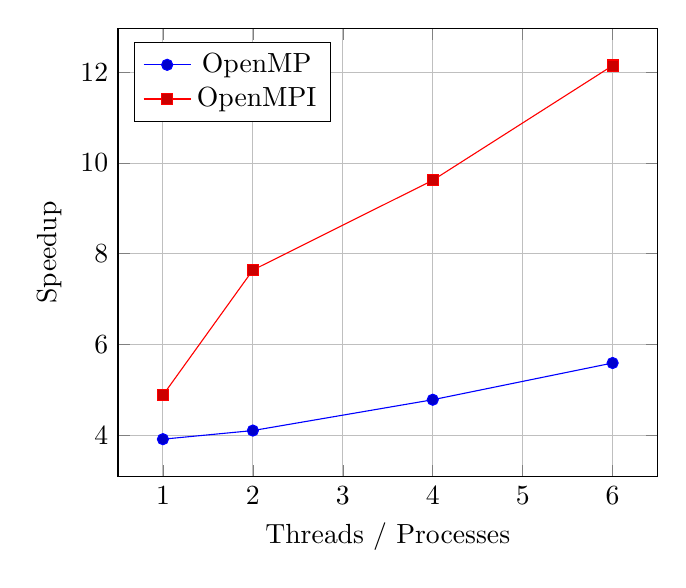
\begin{tikzpicture}
\begin{axis}[
    xlabel={Threads / Processes},
    ylabel={Speedup},
    legend pos=north west,
    grid=both,
]
\addplot coordinates {(1,3.91) (2,4.10) (4,4.78) (6,5.59)};
\addlegendentry{OpenMP}
\addplot coordinates {(1,4.88) (2,7.64) (4,9.62) (6,12.15)};
\addlegendentry{OpenMPI}
\end{axis}
\end{tikzpicture}
\caption{Speedup vs. Parallelism}
\end{figure}

\begin{figure}[h]
\centering
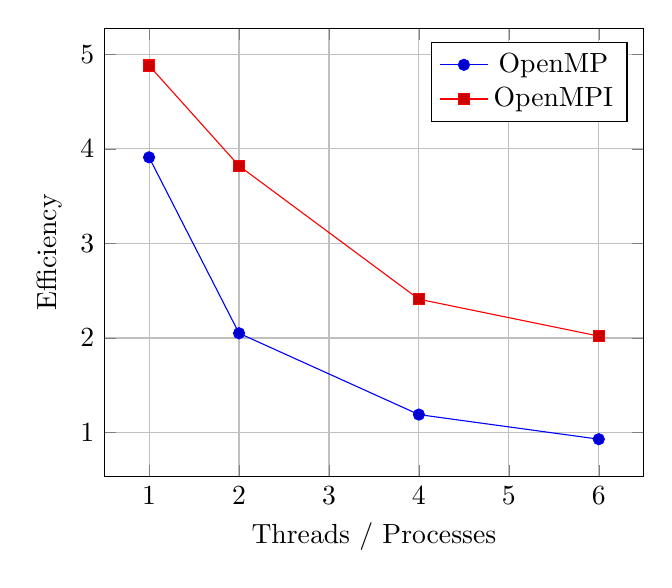
\begin{tikzpicture}
\begin{axis}[
    xlabel={Threads / Processes},
    ylabel={Efficiency},
    legend pos=north east,
    grid=both,
]
\addplot coordinates {(1,3.91) (2,2.05) (4,1.19) (6,0.93)};
\addlegendentry{OpenMP}
\addplot coordinates {(1,4.88) (2,3.82) (4,2.41) (6,2.02)};
\addlegendentry{OpenMPI}
\end{axis}
\end{tikzpicture}
\caption{Efficiency vs. Parallelism}
\end{figure}

\FloatBarrier

\section{Parallelism Conclusions Based on \\Amdahl's Law (Strong Scaling)}

From the measured 1 million tuple dataset runs, the OpenMP implementation reached it's optimal speedup at six threads, however reached it's maximum efficiency at 1 thread. Similarly, OpenMP showcased increasing speedup as the process count grew (more substantial of a curve than OpenMP), however showed a declining efficiency. This aligns  with Amdhal's law, which states that while parallel performance improves initially, it diminishes due to serial portions and synchronization overhead. Therefore, the optimal thread configuration is likely a lower thread count, likely around 2-3, where speedup remains significant while efficiency is not too degraded.

\section{Program Scaling with Thread Count (Weak Scaling)}

To answer this question, scaled small datasets (50{,}000, 100{,}000, 200{,}000, 300{,}000) were generated and paired with the thread counts of 1, 2, 4, and 6. Additionally, sequential executions are noted for reference. Below are the results:

\begin{center}
\begin{tabular}{c c c c c}
\hline
\textbf{Threads/Processes} &
\textbf{Problem Size} &
\textbf{Serial (s)} &
\textbf{OpenMP (s)} &
\textbf{OpenMPI (s)} \\
\hline
1 & 50{,}000  & .0136 & .0279 & .0161 \\
2 & 100{,}000 & .1504 & .0693 & .0363 \\ 
4 & 200{,}000 & .3295 & .1483 & .0643 \\
6 & 300{,}000 & .4509 & .2008 & .1259 \\
\hline
\end{tabular}
\end{center}

\begin{figure}[h]
\centering
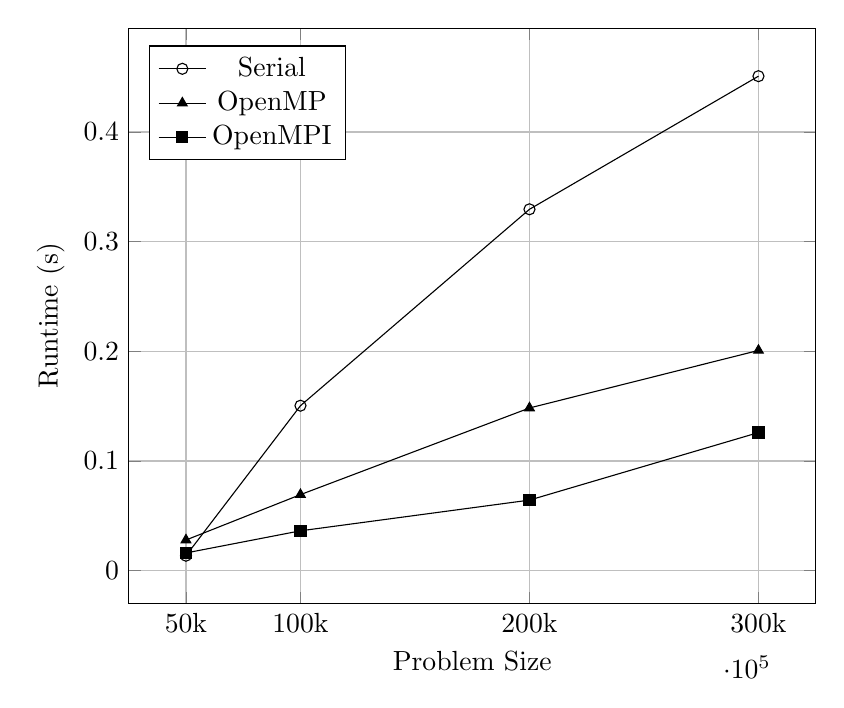
\begin{tikzpicture}
\begin{axis}[
    xlabel={Problem Size},
    ylabel={Runtime (s)},
    xtick={50000,100000,200000,300000},
    xticklabels={50k,100k,200k,300k},
    legend pos=north west,
    grid=both,
    width=0.85\linewidth,
]
\addplot[
    mark=o
] coordinates {
    (50000,0.0136)
    (100000,0.1504)
    (200000,0.3295)
    (300000,0.4509)
};
\addlegendentry{Serial}

\addplot[
    mark=triangle*
] coordinates {
    (50000,0.0279)
    (100000,0.0693)
    (200000,0.1483)
    (300000,0.2008)
};
\addlegendentry{OpenMP}

\addplot[
    mark=square*
] coordinates {
    (50000,0.0161)
    (100000,0.0363)
    (200000,0.0643)
    (300000,0.1259)
};
\addlegendentry{OpenMPI}

\end{axis}
\end{tikzpicture}
\caption{Runtime growth relative to increasing problem size under weak scaling.}
\end{figure}

\FloatBarrier

In an ideal weak-scaling scenario, runtimes would remain constant while problem size and threads proportionally increase (which they do in this scenario). This is supported by the control serial implementation, which roughly grows linearly. However, the parallel programs do not remain flat, having a small linear increase in rumtime as problem size/threads increase. This points to potential weak-scaling degradation.

\section{Conclusions}

From these performance results, we can clearly see that both OpenMP and MPI parallel implementations are more efficient than the serial implementations, showing better weak and strong scaling. However, it is clear that the \textbf{MPI} implementation is the fastest and most optimized within our scenario.

\end{document}
